\documentclass[11pt]{article}
\setlength{\parskip}{.08in} 
\renewcommand\arraystretch{1.2}
\usepackage{commath}
\usepackage{listings}
\usepackage{hyperref} 
\setlength{\parindent}{0in}

\lstdefinestyle{mystyle}{
basicstyle=\fontsize{12}{9}\selectfont\ttfamily
}
\lstset{style=mystyle}

% Added packages
\usepackage{setspace}
\usepackage{enumerate}
\usepackage{bm}
\usepackage{amsmath}
\makeatletter
\renewcommand*\env@matrix[1][\arraystretch]{%
  \edef\arraystretch{#1}%
  \hskip -\arraycolsep
  \let\@ifnextchar\new@ifnextchar
  \array{*\c@MaxMatrixCols c}}
\makeatother
%\usepackage[dvips, bookmarks, colorlinks=true, plainpages = false, 
%citecolor = green, urlcolor = blue, filecolor = blue] {hyperref}
%\usepackage[font=small,format=plain,labelfont=bf,up,textfont=it,up]{caption}

% Set the beginning of a LaTeX document
\usepackage{graphicx}
\graphicspath{ {./images/} }

%\usepackage{endnotes}
%\let\footnote=\endnote

\usepackage{titlesec}
\titleformat{\section}
  {\normalfont\fontfamily{phv}\fontsize{14}{17}\selectfont}{\thesection}{1em}{}

\oddsidemargin 0.25in
\evensidemargin 0.25in 

\headheight 0.0in
\headsep 0.0in
\topmargin -0.25in

\textwidth 6.0in 
\textheight 9.0in 

\paperheight 11.0in
\paperwidth 8.5in

\begin{document}

\title{Analysis of the Ecological Impact of Homo Necrosis}         % Enter your title between curly brackets
\author{Philippe Nadon}

\date{ \today}          % Enter your date or \today between curly brackets
\maketitle

\footnote{Corresponding author: nadon@ualberta.ca}\\[0.5cm]
{\small Faculty of Science, University of Alberta}\\
{\small Camrose, AB, Canada}\\[0.5cm]

\thispagestyle{empty}

%\onehalfspacing
\doublespacing

\begin{abstract}
In this paper a human-zombie model is used to analyze any equilibrium points in the model, and their type and stability. This topic is of great importance due to a growing concern of the suspiciously zombie-like behaviour of university students during exam times.

\end{abstract}

\textbf{Keywords:} Zombies, Homo Necrosis, Humans, Students, Exams, Ecology

\newpage

\setcounter{page}{1}

\section{Introduction}

The equations which model the relation between the population of zombies and humans are as shown below:
\begin{equation}
\dot{H} = aH(1 - H) - bHZ^2
\end{equation}
\begin{equation}
\dot{Z} = bHZ^2 - cH^3Z
\end{equation}

Where $H$, $Z$ are the populations of humans and zombies respectively, $\dot{H}$, $\dot{Z}$ are the rates of change of these populations, $a$ is the coefficient corresponding to the net birth and death rate of humans, $b$ is the coefficient corresponding to the encounter rate of infectious zombies with humans, and $c$ is the encounter rate of a zombie-hunting squad and zombies.

\subsection{Restrictions} 
In order for this model to make sense, the following restrictions are applied:
\begin{enumerate}
\item $a$, $b$, $c$ $> 0$, this implies humans are not dying of non-zombie causes faster than they are being born, and that humans are not converting zombies back into humans faster than humans are being converted to zombies.
\item $H,Z \geq 0$, a negative population is nonsense.
\end{enumerate}

\subsection{Terms of Equation}
Let's break down the equation term by term:
\begin{enumerate}
\item $aH(1-H)$:\\
This term represents the positive factor of $\dot{H}$, which is the growth of the human population. Since the growth of a population relies on its current size, the coefficient $a$ is multiplied by $H$. However, there is also a carrying capacity $(1 - H$), where the growth rate of humans begins to slow down as the population approaches a limit. In this model, the limit is represented by 1, which means the human population must be $H$ less than 1, otherwise this model wouldn't work. In fact, $H$ can be considered the ratio of the current human population to the maximum human population.
\item $bHZ^2$:\\
This term represents the rate at which the zombie convert humans. The term $HZ^2$ implies that in order to convert one human it would take two zombies. Keep in mind both $H$ and $Z$ are less than 1, so logically the higher number of zombies required to convert a human, the higher the exponent on the $Z$ variable, and thus the lower the value of this term.\\
Notice also that this term appears both in the human growth rate and zombie growth rate equations, this is because the growth in population of zombies is directly dependant on the death of humans by zombie conversion.
\item $-cH^3Z$:\\
This term represents the rate at which the humans kill zombies. Similarly to the previous term, the $H^3Z$ implies that it takes three humans to kill one zombie.
\end{enumerate}

\section{Equilibrium Points}
Finding equilibrium points will help us find trends in the population change, such as which population values the model will approach and remain at based on initial values.\\
An equilibrium point is a point where the rate of change for all variables is $0$. In the case of this model:
\begin{equation}
aH(1 - H) - bHZ^2 = 0
\end{equation}
\begin{equation}
bHZ^2 - cH^3Z = 0
\end{equation}
At this point, since the rate of change is $0$, the populations will remain at this value (realistically they will only oscillate minutely).

\subsection{Trivial Points}
 For starters, there is the trivial solution of $(H, Z) = (0,0)$. This is trivial because it makes sense that if there are no zombies or humans around then their growth rate will remain 0, since our model does not depict zombies or humans spontaneously growing out of nothing.\\
Another trivial solution would be at $(H, Z) = (1, 0)$. At this point the zombie population would be gone and so they would be unable to convert any more humans. Humans would have reached carrying capacity and would be unable to grow larger but also would have no zombies reducing their population. Thus both the human population and the zombie population would remain constant.\\ 

\subsection{Non-trivial Points, $H,Z > 0$}
The more interesting equilibrium points we can analyze are the non-trivial points, which are less obvious and require more calculations to find.\\
Let's start by manipulating equations (3) and (4) to obtain the equilibrium points $H_e, Z_e$:
\begin{equation}
aH_e(1 - H_e) - bH_eZ^2 = H_e(a(1 - H_e) - bZ^2) = 0
\end{equation}
\begin{equation}
bH_eZ_e^2 - cH_e^3Z_e = H_e(bZ_e^2 - cH_e^2Z_e) = 0
\end{equation}
since $H,Z > 0$, we can divide $H_e$ on both sides for both equations:\\
From equation (6):
\[bZ_e^2 = cH_e^2Z_e \]
\begin{equation}
Z_e = \frac{c}{b} H_e^2 
\end{equation}
Inserting this result in (5):
\begin{equation}
a(1 - H_e) = bZ_e^2 = \frac{c^2}{b}H_e^4
\end{equation}

\section{ Stability of Non-trivial Equilibrium Point}
Now, we will find the Jacobian and then use Matlab to compute the coordinates of the non-trivial equilibrium point, and its stability. This will allow us to find if there is a population size of humans and zombies where neither species is overtaking the other, and whether we will naturally approach this point or one of the two trivial points (extinction of both species or extinction of zombies).

\subsection{Jacobian}
The Jacobian of equations (1) and (2) is defined as the following:

\[
det \abs{
\begin{bmatrix}[1.5]
\frac{d \dot{H}}{dH} && \frac{ d \dot{H} }{ dZ} \\
\frac{d \dot{Z}}{dH} && \frac{ d \dot{Z} }{ dZ} \\
\end{bmatrix} 
 - \lambda I}
 =
 det \abs{
\begin{bmatrix}[1.5]
a - 2a H_e - b Z_e^2 && -2b H_e Z_e \\
b Z_e^2 - 3c H_e^2 Z_e && 2b H_e Z_e - c H_e^3 \\
\end{bmatrix} 
 - \lambda I}
\]

Substituting for $Z_e$ gives us

\begin{equation}
det \abs{
\begin{bmatrix}[1.5]
a - 2aH_e - \frac{c^2}{b}H_e^4 && -2cH_e^3 \\
\frac{c^2}{b}H_e^4 - 3 \frac{c^2}{b}H_e^4&& 2cH_e^3 - cH_e^3 \\
\end{bmatrix} 
 - \lambda I}
 =
 det \abs{
\begin{bmatrix}[1.5]
-aH_e && -2cH_e^3 \\
-2 \frac{c^2}{b} H_e^4 && cH_e^3 \\
\end{bmatrix} 
 - \lambda I}
\end{equation}

Finally, evaluating the above equation gives us

\[
(-aH_e - \lambda)(cH_e^3 - \lambda) - (-2 \frac{c^2}{b} H_e^4)(-2cH_e^3)
\]

Which can be simplified to

\begin{equation}
(\lambda + a H_e) (\lambda - c H_e^3 ) - 4 \frac{c^3}{b} H_e^7
\end{equation}

Beyond this point, solving through numerical methods using Matlab will become the preferred tool of choice.

\subsection{ Direction Field}
We can find the direction field for the system of ODEs in equations (7) and (8) by running the following code and plotting it in Matlab:

\begin{lstlisting}[language = Matlab]
global a b c;
a = 1;
b = 1;
c = 1;

function [ret] = hPopRate( H, Z) 
global a  b;
ret = a.*H.*(1 - H) - b.*H.*Z.^2;
end

function [ret] = zPopRate( H, Z)
global b c;
ret = b.*H.*Z.^2 - c.*H.^3.*Z;
end

function [] = plotDirectionField()
[H,Z] = meshgrid( 0: 0.01: 1.0, 0: 0.01: 2.0);
quiver( H, Z, hPopRate( H, Z), zPopRate( H, Z));
end
\end{lstlisting}

This code plotted the following direction field:\\
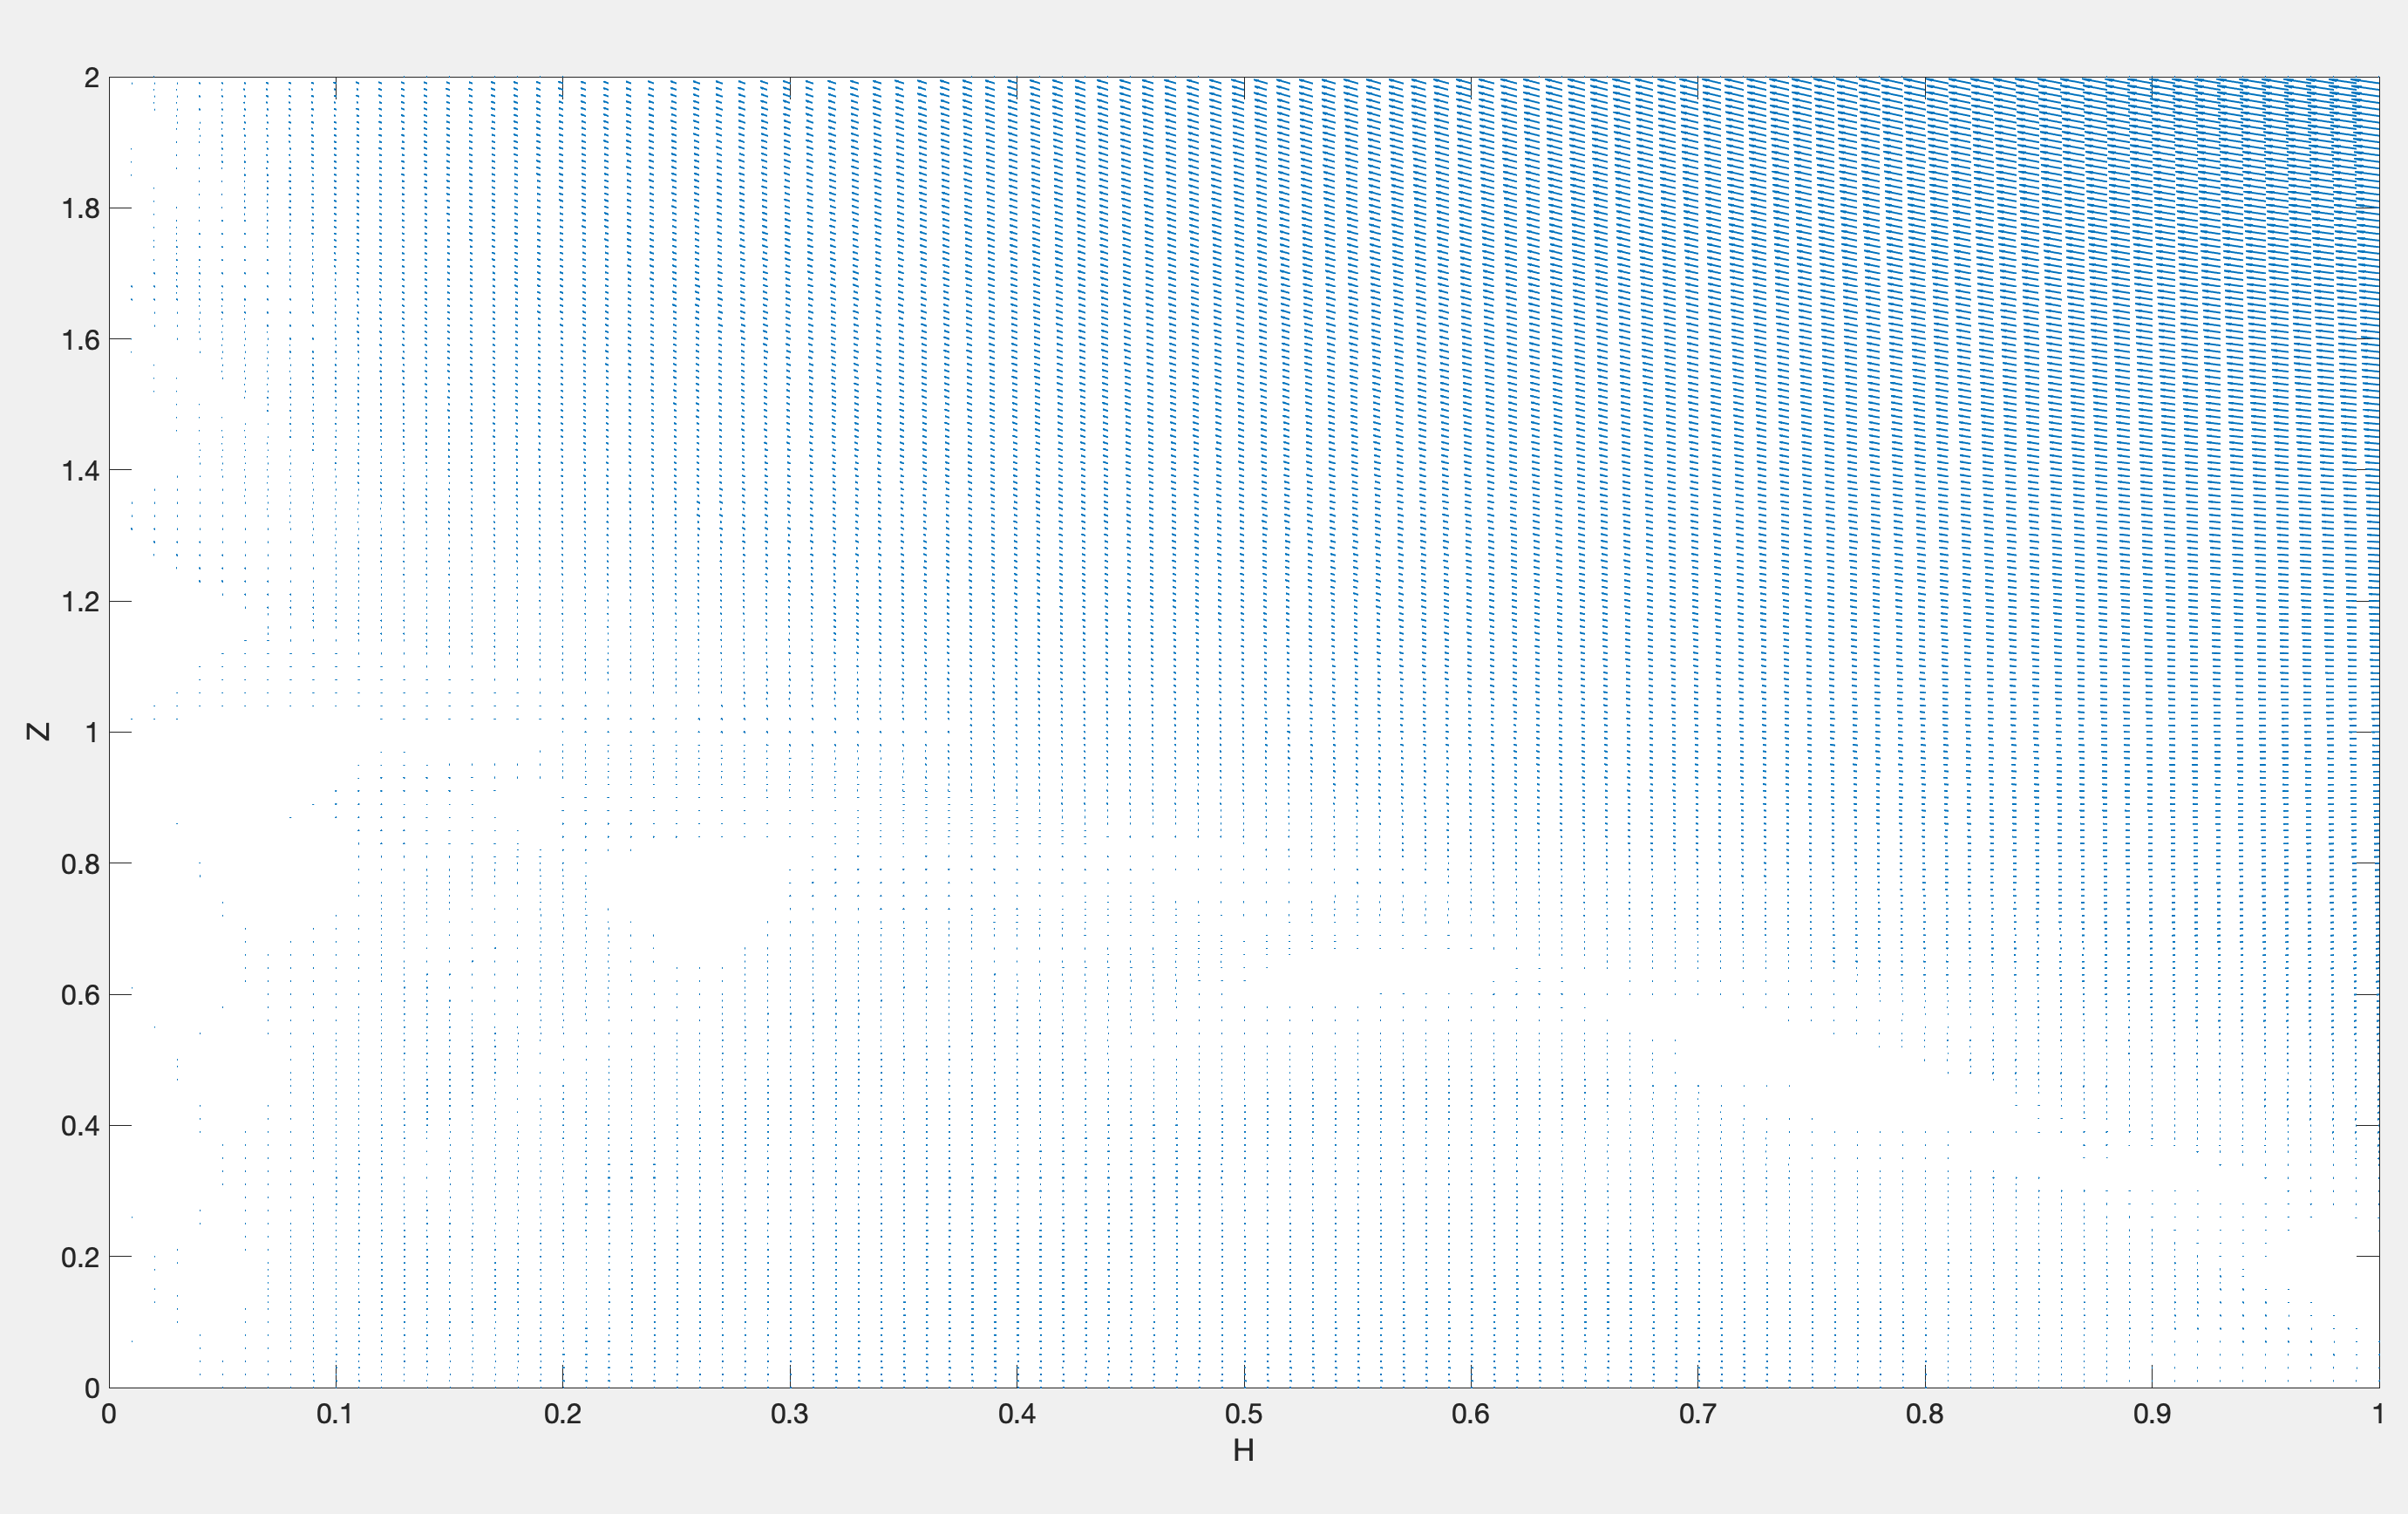
\includegraphics[scale = 0.32]{Q5.png}

From this graph we can estimate the non-trivial equilibrium point to be around $H = 0.7$, which will allow us to use an educated guess to start with when we numerically computer the equilibrium point in the next section.

\subsection{ Non-trivial Coordinates}
Now that we have a vague estimation of the non-trivial equilibrium point, we can compute a far more accurate result using more Matlab code:

\begin{lstlisting}[language = Matlab]
function [ret] = hEqFunc( H)
global a b c;
ret = a.*(1 - H) - c.^2/b.*H.^4;
end

function [ret] = zEqFunc( H_e)
global b c;
ret = c*H_e^2/b;
end

function [H_e, Z_e] = computeCoordinates( guessH)
H_e = fzero( @hEqFunc, guessH);
Z_e = zEqFunc( H_e);
end
\end{lstlisting}

This will tell us at what values of $H$ and $Z$ can we expect a fixed balance between human and zombie populations. After running the computation we received a result of:
\begin{equation}
H = 0.7245, Z = 0.5249
\end{equation}

We can verify by inserting these values back into the equation:
\begin{equation}
\dot{H} = aH(1 - H) - bHZ^2 = 0.7245*(1 - 0.7245) - 0.7245*0.5249^2 = 0
\end{equation}

\begin{equation}
\dot{Z} = bHZ^2 - cH^3Z = 0.7245*0.5249^2 - 0.7245^3*0.5249 = 0
\end{equation}

If you input these values yourself to see if they equal zero, you will be disappointed to find that they don't. This is an expected result of using numerical computation. All computers have a limited amount of memory and processing power, and so the "correct" answer is an answer which is deemed to be accurate enough for your needs. In this case, 4 significant digits is enough accuracy for this paper.

\subsection{ Type and Stability of Equilibrium Point}
Another point of interest is whether or not that point is stable, and what type it is. This will aid us in understanding the behaviour of this model as the human and zombie population changes. Here is the Matlab code which finds the eigenvalues:

\begin{lstlisting}[language = Matlab]
global H_eGuess;
H_eGuess = 0.7;

function [matrixHZ] = makeJacobian()
global a b c H_eGuess;
[H_e, ~] = computeCoordinates( H_eGuess);
matrixHZ = [-a*H_e, -2*c*H_e^3 ; -2*c^2/b*H_e^4, c*H_e^3];
end

function [ eigs] = computeEigenvalues()
matrixHZ = makeJacobian();
eigs = eig( matrixHZ);
end
\end{lstlisting}

After running the computation the answer it found was 

\begin{equation}
\lambda_1 = -1.0231, \lambda_2 = 0.6789
\end{equation}

which means the equilibrium point is a saddle point, due to both eigenvalues being real, and only one being less than zero.

\section{Further Tests}
We have determined the type, location, and stability of the non-trivial equilibrium point, but there are still areas which should be analyzed, such as the model's sensitivity to change in initial conditions, and a more visual representation of the equilibrium point by plotting multiple cases with slightly varying initial conditions.

\subsection{Sensitivity of Initial Conditions}
Now we will compare the change in our model's behaviour based on the initial conditions given to it. This will help us understand any form of "butterfly effect" we might get based on the conditions we start with. We will test this by comparing the initial conditions
\[
t0=0.0, H_0=0.1, Z_0=0.357 
\]
with
\[ 
t_0=0.0, H_0=0.1, Z_0=0.358
\]
With step size $h = 0.001$ and number of steps $N=20'000$.

Here is the code which computes and plots the graphs:

\begin{lstlisting}[language = Matlab]
global stepSize numSteps;
stepSize = 0.001;
numSteps = 20000;

plotGraphs( [ 0.0, 0.1, 0.357 ; 0.0, 0.1, 0.358]);

function [retH, retZ, retT] = eulerMethod( h, z, t)
global stepSize;
retH = h + stepSize*hPopRate( h, z);
retZ = z + stepSize*zPopRate( h, z);
retT = t + stepSize;
end

function [] = plotGraphs( initConds)
global numSteps;

for i = 1:( size( initConds, 1))
t=linspace(1,numSteps);
h=linspace(1,numSteps);
z=linspace(1,numSteps);

% First entry
t(1)=initConds(i,1);
h(1)=initConds(i,2);
z(1)=initConds(i,3);

% Euler method
for j = 1:(numSteps-1)
   [h(j+1), z(j+1), t(j+1)] = eulerMethod( h(j), z(j), t(j));
end

% Plotting the solution
plotTitle = [ 'Initial H = ', num2str( h(1)),...
    ', Initial Z = ', num2str( z(1))];
figure('Name', plotTitle,'NumberTitle','off');
plot(t,h,'*');
hold on
plot(t,z,'x');
hold off
end
end
\end{lstlisting}

\newpage
Below we can see the graph corresponding to the initial condition $H = 0.1$, $Z = 0.357$:

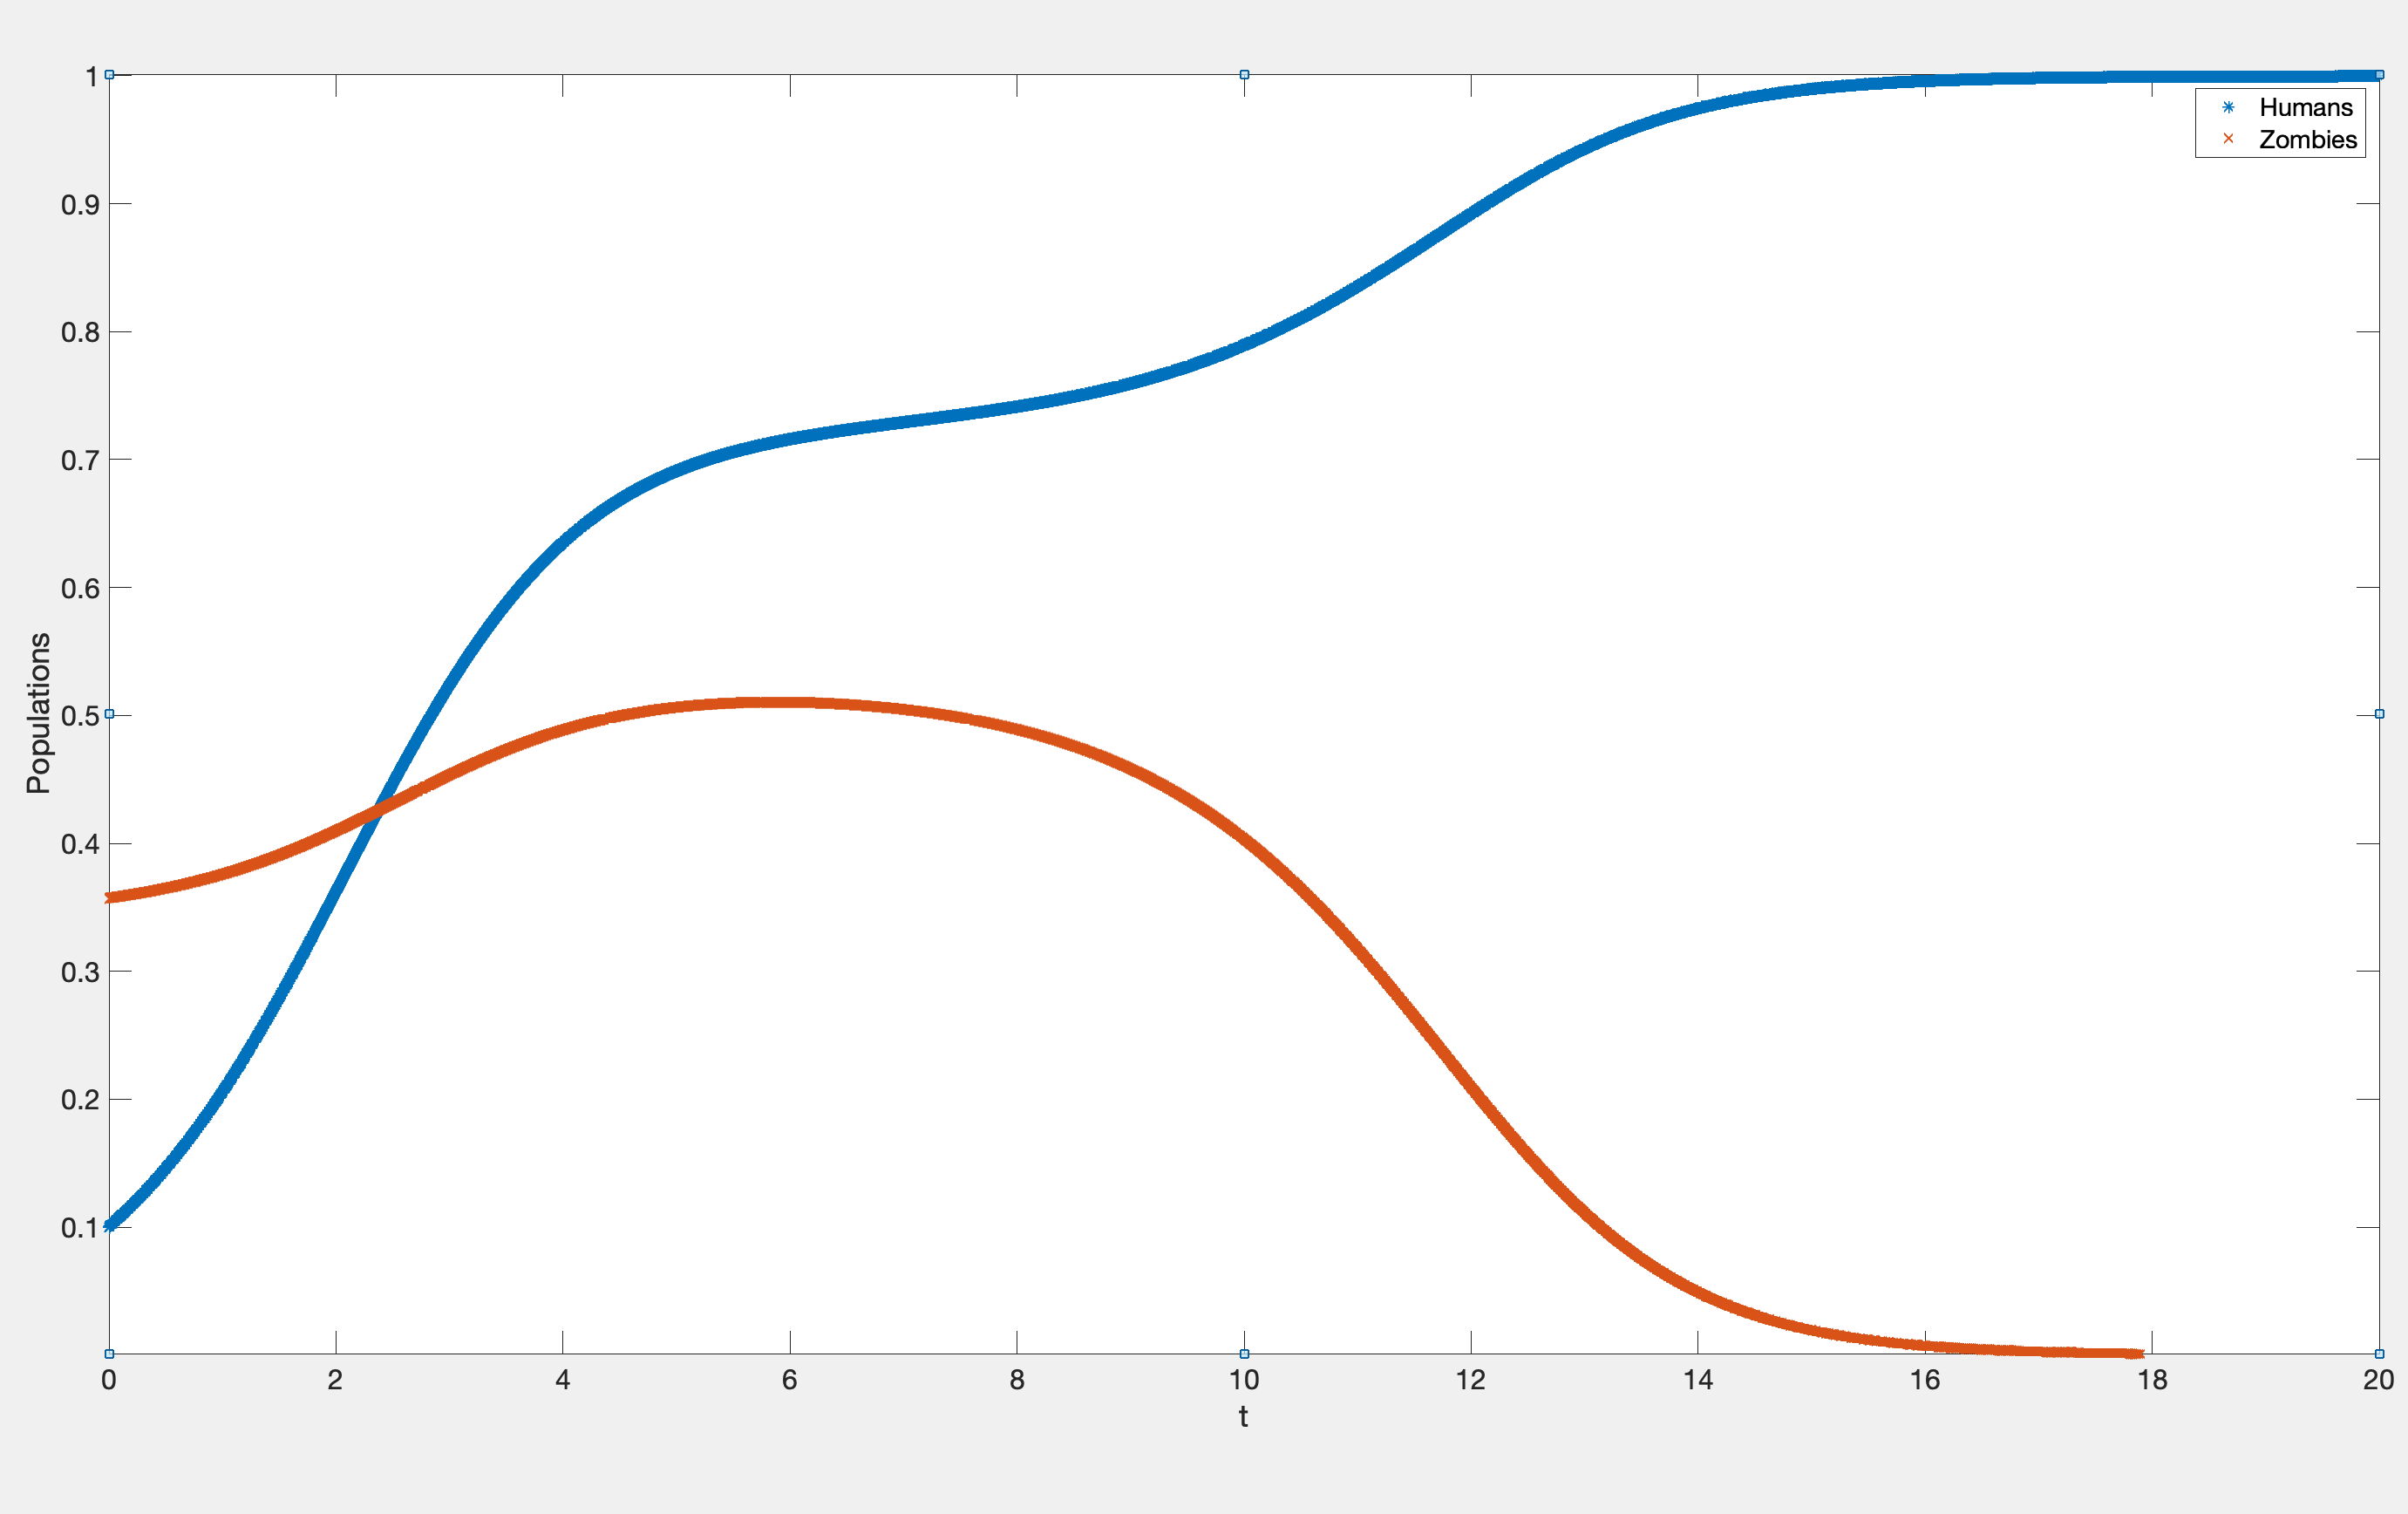
\includegraphics[scale = 0.32]{Q81.png}

And below is the graph corresponding to the initial conditions $H = 0.1$, $Z = 0.358$:

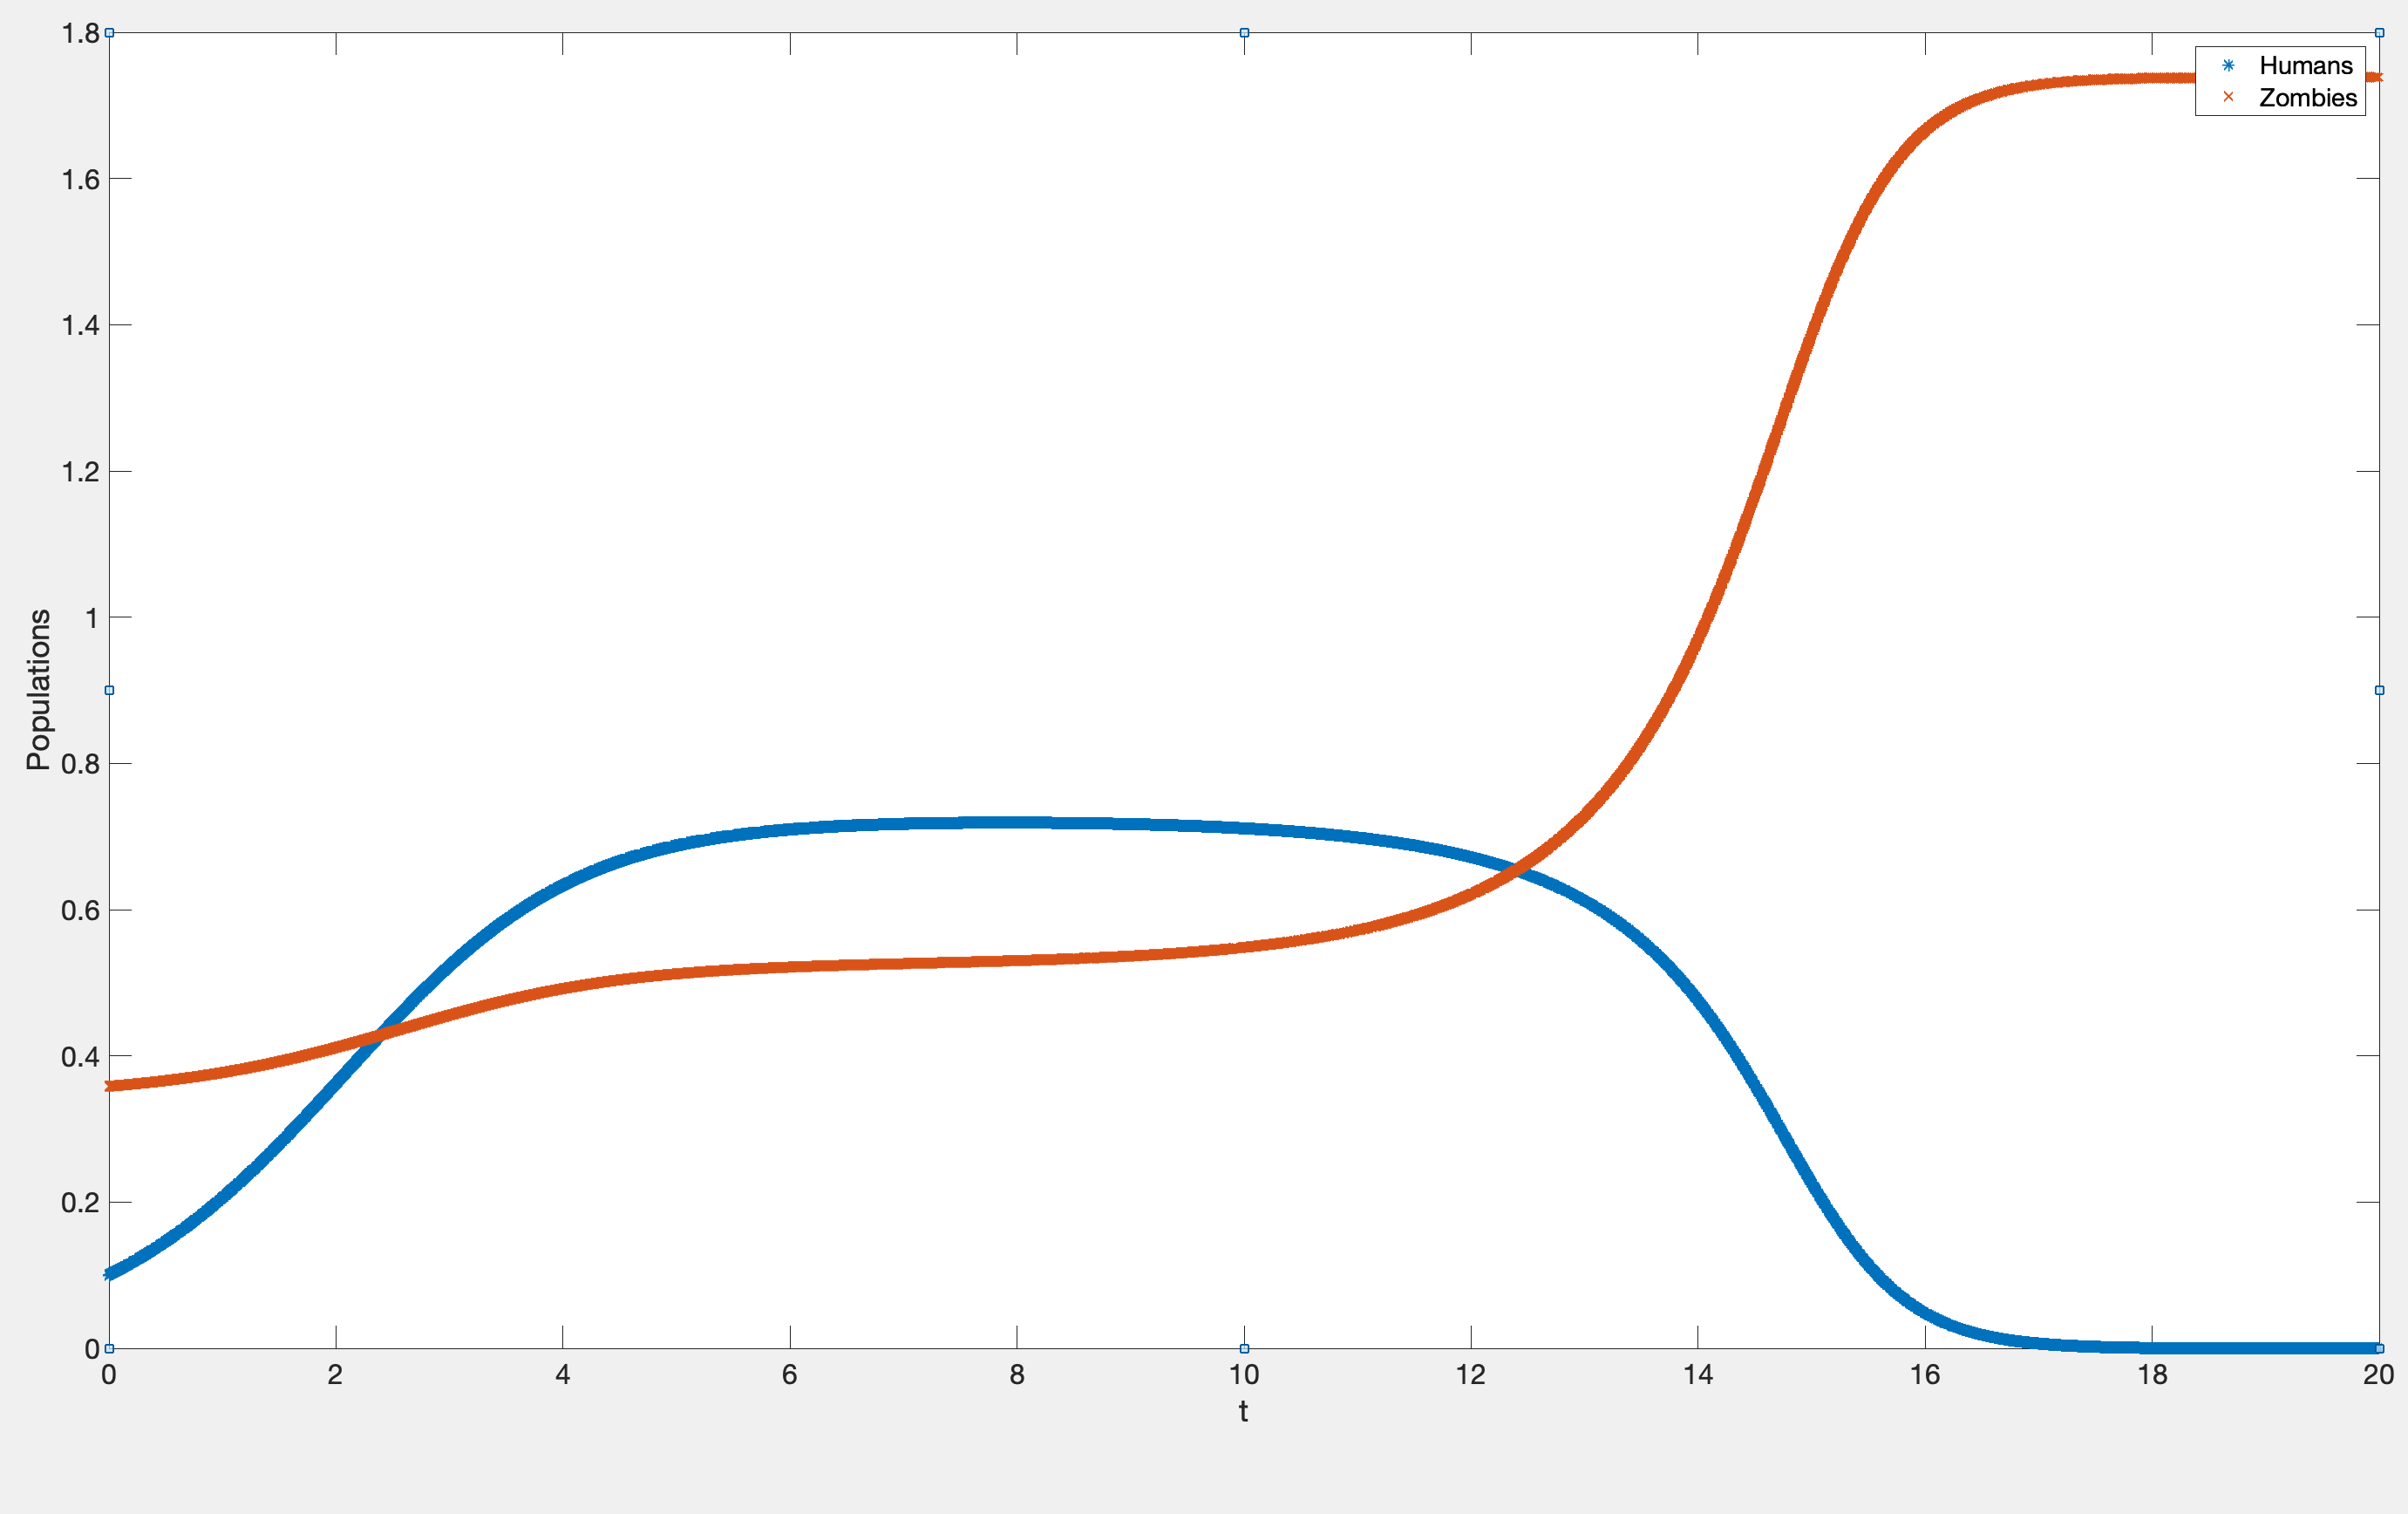
\includegraphics[scale = 0.32]{Q82.png}

We can see that with just a slight variation in the initial population of zombies, that our race can either survive and overcome the outbreak of zombies, or we will temporarily overtake them before eventually being overwhelmed. It is interesting to note that the change in the population of zombies seems contrast directly with the change in human population, albeit lagging slightly behind. In both graphs the zombie and human populations initially rise to a higher population, after which the effects of the human population relative to its carrying capacity causes its growth to slow down, and then the two populations begin to directly compete with each other.

\subsection{ Visual of Equilibrium Point}
Lastly before the conclusion, we will create a more visual representation of the saddle-point of our equilibrium, by plotting multiple equations on the same plot, each of which vary by slightly different initial conditions. Below are the code and graphs corresponding to this problem:

\begin{lstlisting}[language = Matlab]
plotPhaseGraphs( [ 0.0, 0.1, 0.357 ; 0.0, 0.1, 0.358 ;...
    0.0, 0.99, 0.64 ; 0.0, 0.99, 0.65]);

function [] = plotPhaseGraphs( initConds)
global numSteps;

for i = 1:( size( initConds, 1))
t=linspace(1,numSteps);
h=linspace(1,numSteps);
z=linspace(1,numSteps);

% First entry
t(1)=initConds(i,1);
h(1)=initConds(i,2);
z(1)=initConds(i,3);

% Euler method
for j = 1:(numSteps-1)
   [h(j+1), z(j+1), t(j+1)] = eulerMethod( h(j), z(j), t(j));
end

% Plotting the solution
plot(z,h,'*');
hold on
end
hold off
end
\end{lstlisting}

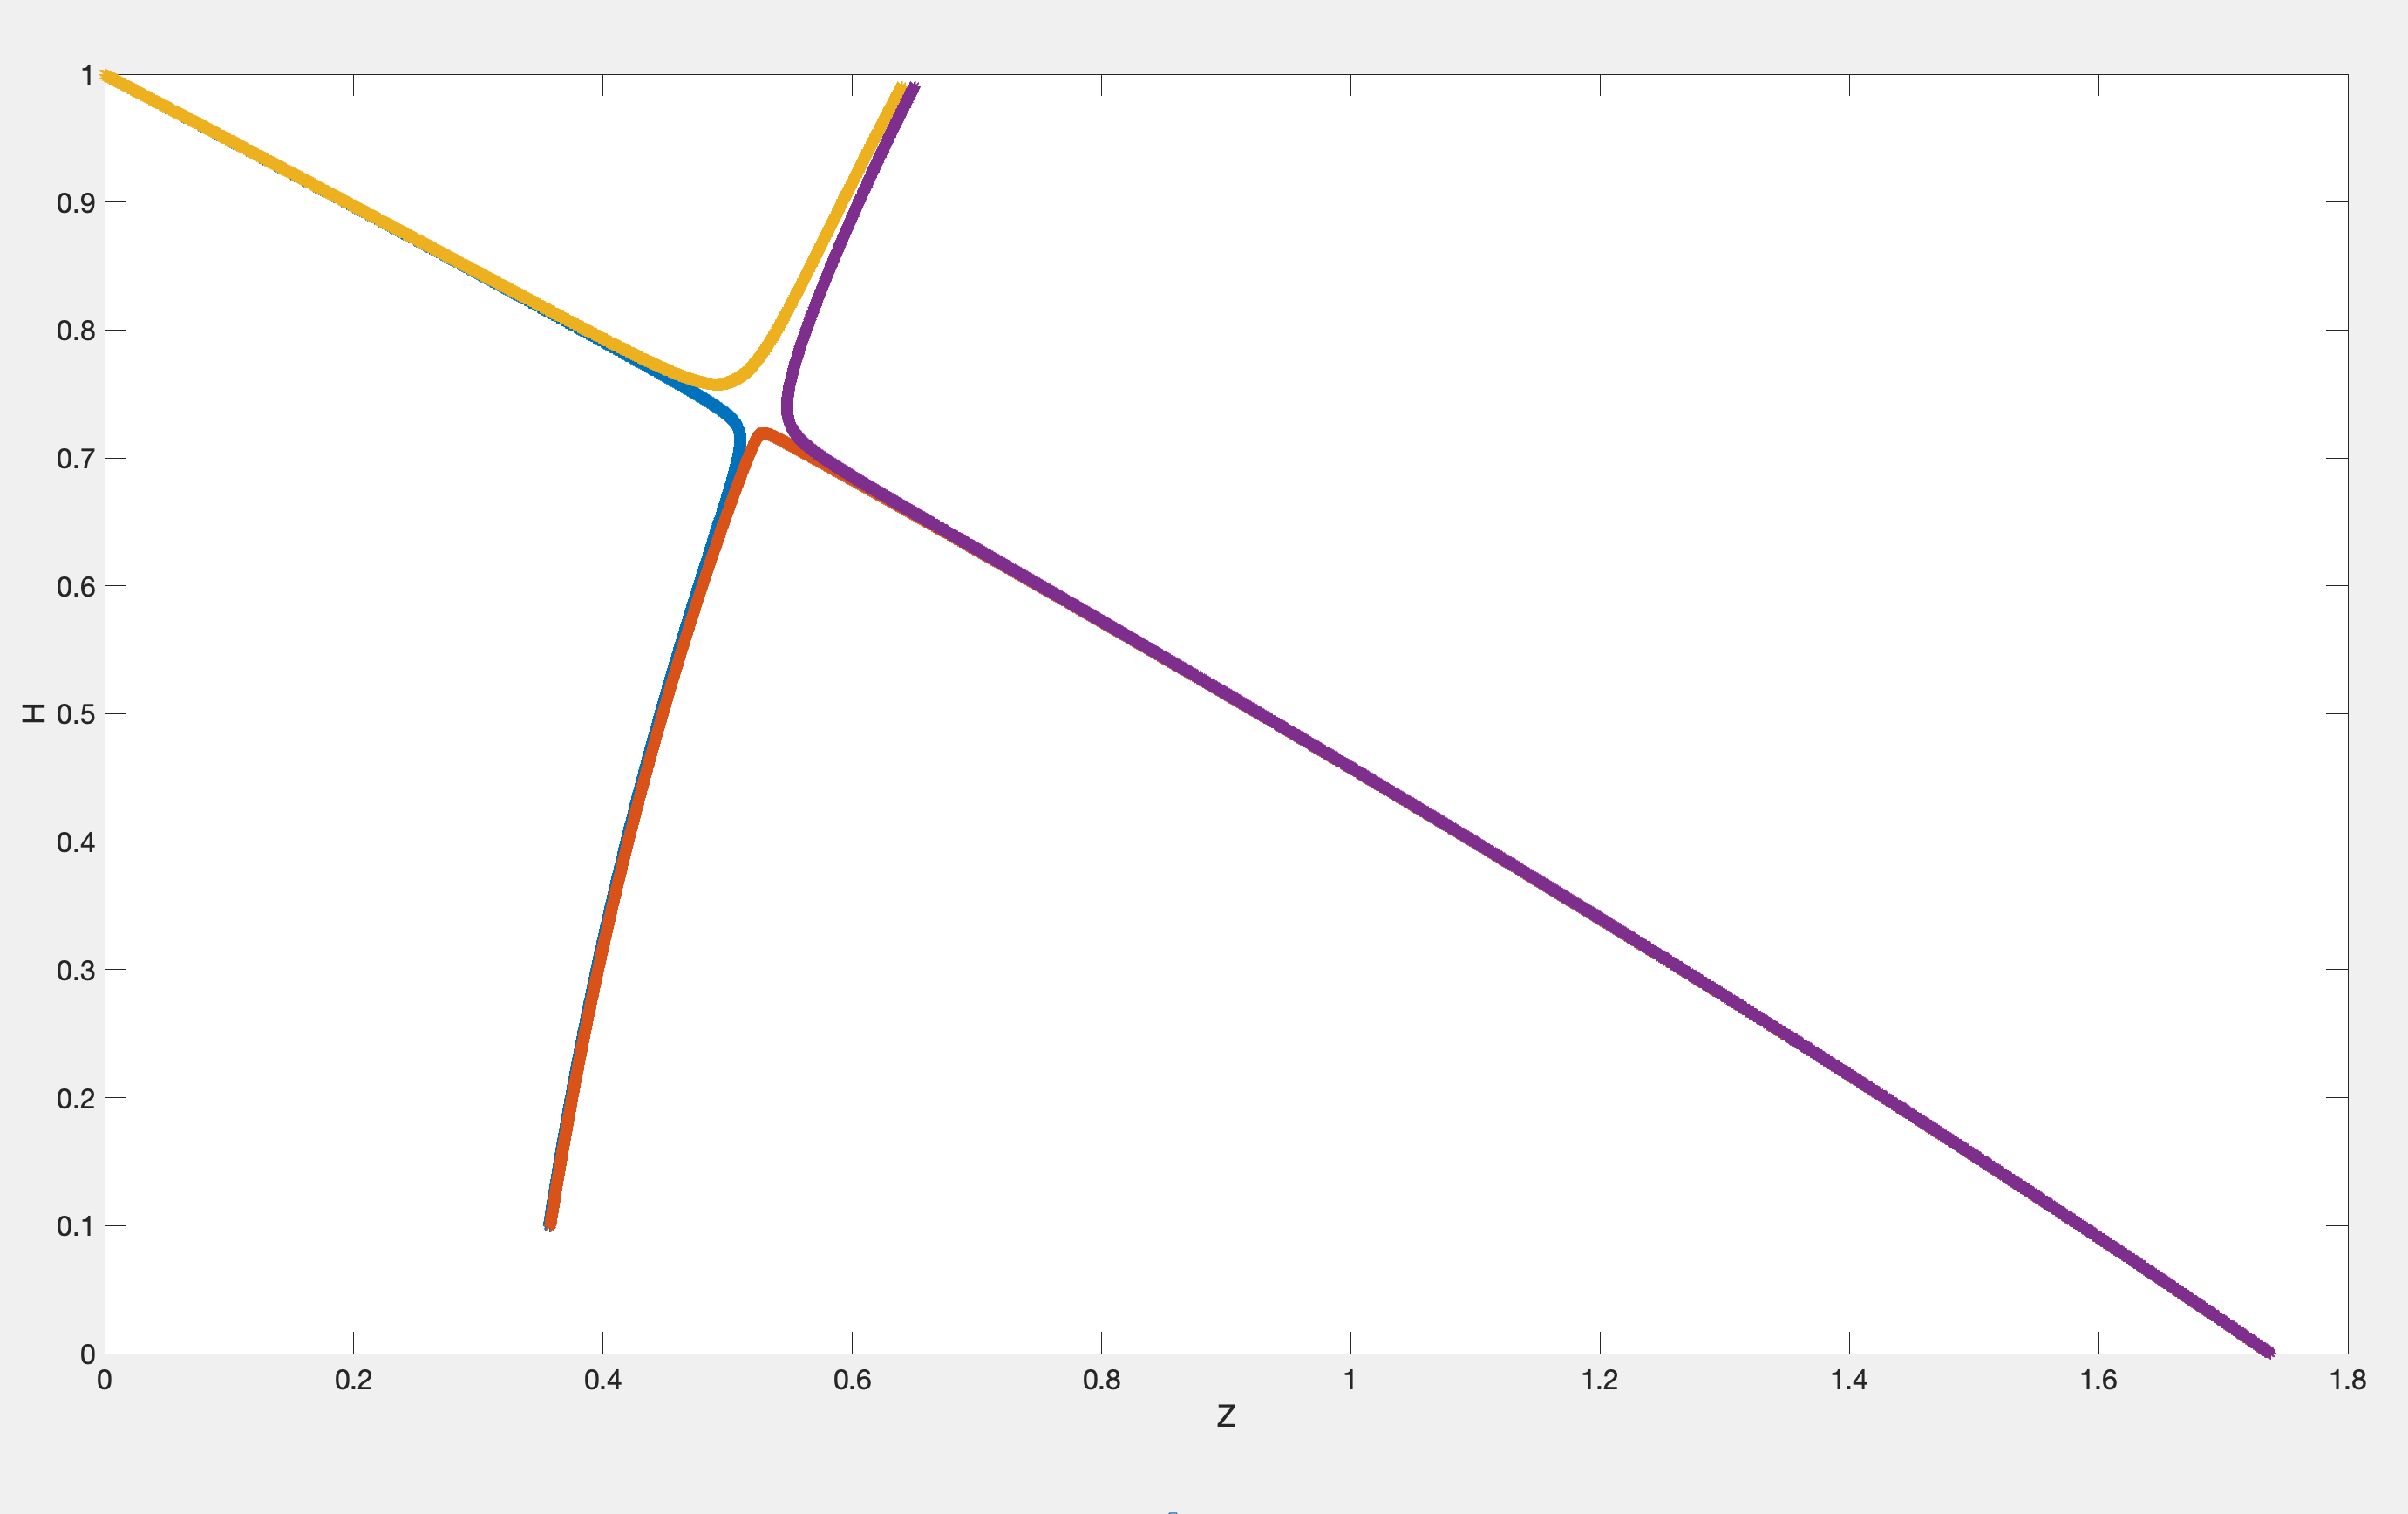
\includegraphics[scale = 0.32]{Q9.png}

This plot demonstrates the equilibrium point's instability, since each of the four lines within this plot approach the equilibrium point at $H = 0.7245, Z = 0.5249$, but then turn and move away, thus visually demonstrating that it is a saddle point.

\section{Conclusion}

As the above graphs and calculations have shown, our relation with zombies is unstable, meaning that there is no equilibrium point we will inevitably approach. Rather, the outcome is highly sensitive to the initial conditions presented to this model, meaning that the difference between humans eradicating the zombies, and the zombies converting us all is very fine, and could switch with only a slight oscillation, such as humans suddenly catching a flu, which will slightly decrease our numbers. Predicting an outcome of a zombie apocalypse would be nigh impossible due to the instability of the equilibrium, and the butterfly effect of the initial variables.

\textbf{Make sure to look at and test the source code at \href{https://bit.ly/2TLMNfn}{https://bit.ly/2TLMNfn}}

\end{document}


